% 05_results.tex - the output files, the water balance check and the plots
\section{Read the results}

\step{List the output files}
\term{t1_ls_out.txt}
\why the folder holds:
\begin{itemize}
\item Raven's usual files: \cmd{Hydrographs.csv}, \cmd{Diagnostics.csv}, \cmd{WatershedStorage.csv}, \cmd{solution.rvc}
  and others;
\item four groundwater files of a coupled run: \cmd{GWModelSummary.txt}, \cmd{GWBudget.csv}, \cmd{GWHRUState.csv} and
  \cmd{GWConnectivity.csv}.
\end{itemize} The folder \cmd{out/mf6/} holds the MODFLOW~6 model that Raven built
and ran. You can open it with FloPy (a Python package for MODFLOW) or with ModelMuse (a graphical MODFLOW program).

\step{Read what Raven built}
\cmd{GWModelSummary.txt} describes the groundwater model. Show its first lines:
\term{t1_summary.txt}
\why Raven laid a regular grid of \V{t1:nlay}~layers, \V{t1:nrow}~rows and \V{t1:ncol}~columns of \V{t1:cell}~m cells
over the \V{t1:nhru} coupled HRUs (the HRUs that have groundwater). It kept the \V{t1:activecols} columns of cells that lie
under these HRUs (the \emph{active} columns) and placed \V{t1:rivcells} river cells along the river lines. The second part
of the file (not shown) lists every coupled HRU, with its area in \cmd{Liard.rvh}, the area of its polygon and the number
of cells it covers.

\step{Read the groundwater budget}
\cmd{GWBudget.csv} has one line per day and \V{t1:ncolsBudget} columns. Show the first columns of the first lines:
\term{t1_budget_head.txt}
\why every flow is in m\textsuperscript{3}/d for the whole groundwater model. The most important columns are:
\begin{center}\small
\begin{tabularx}{\linewidth}{>{\raggedright\arraybackslash}p{0.33\linewidth}X}\toprule
Column & Meaning (and the mean of this run)\\\midrule
\cmd{Raven recharge}, \cmd{MF6 recharge} & the water that Raven's processes put into its \cmd{GROUNDWATER} store, and what
  MODFLOW received. The two are equal (\V{t1:rech} million m\textsuperscript{3}/d).\\
\cmd{seepage to Raven} & groundwater that seeps out where the water table reaches the model top. It goes back to Raven's
  lowest soil layer (\V{t1:seep} million m\textsuperscript{3}/d).\\
\cmd{storage release} & water released from aquifer storage. Positive means the aquifer drains
  (\V{t1:stor} million m\textsuperscript{3}/d).\\
\cmd{MF6 balance error} & MODFLOW's own balance error, in m\textsuperscript{3}/d and in \% (largest: \V{t1:balerr}~\%).\\
\cmd{outer iterations}, \cmd{converged} & how many iterations MODFLOW needed (at most \V{t1:maxouter}) and whether it
  converged (1 = yes).\\
\cmd{river leakage to aquifer}, \cmd{aquifer discharge to rivers} & the exchange with the river cells
  (\V{t1:fromriv} and \V{t1:toriv} million m\textsuperscript{3}/d). Raven takes this water from its river reaches or adds
  it to them.\\\bottomrule
\end{tabularx}\end{center}
Wells, head boundaries, water-table evaporation, surface stores, reservoirs and the soil zone have columns of their own.
They are zero in this example.

\step{Read the water table under each HRU}
\term{t1_hrustate_head.txt}
\why \cmd{GWHRUState.csv} has, for every coupled HRU, the mean head (\cmd{head\_ID}) and the mean depth of the water table
below the land surface (\cmd{wtdepth\_ID}) of the cells under the HRU. In this run the mean depths go from
\V{t1:wtmin}~m to \V{t1:wtmax}~m.

\step{Check the water balance}\label{st:audit}
The script \cmd{tools\_audit.py} checks every balance of a coupled run. Give it the output folder:
\term{t1_audit.txt}
\begin{tocheck}
\begin{itemize}
\item \cmd{recharge: (Raven - MF6 - dStore - toCHD)/Raven} is 0: all the recharge reached MODFLOW.
\item \cmd{MF6 cumulative residual / gross flow} is very small (here \V{t1:auditRes}).
\item \cmd{unconverged steps} is \V{t1:auditUnconv} and \cmd{ERROR lines} is 0.
\item The river lines (\cmd{river: ...}) are at round-off level (about $10^{-10}$ or smaller).
\item \cmd{Raven MB error max [mm]} is Raven's own water-balance error (\V{t1:auditMB}~mm here).
\end{itemize}
\end{tocheck}

\step{Plot the results}
The script \cmd{plot\_gw.py} draws the budget, the water table and a map:
\term{t1_plot.txt}
\see a summary of the run and the names of the pictures it wrote into \cmd{out/}. Open them with an image viewer. On WSL,
\cmd{explorer.exe out} opens the folder in Windows. Figures~\ref{fig:t1budget} to~\ref{fig:t1map} show them.
\begin{figure}[!htbp]\centering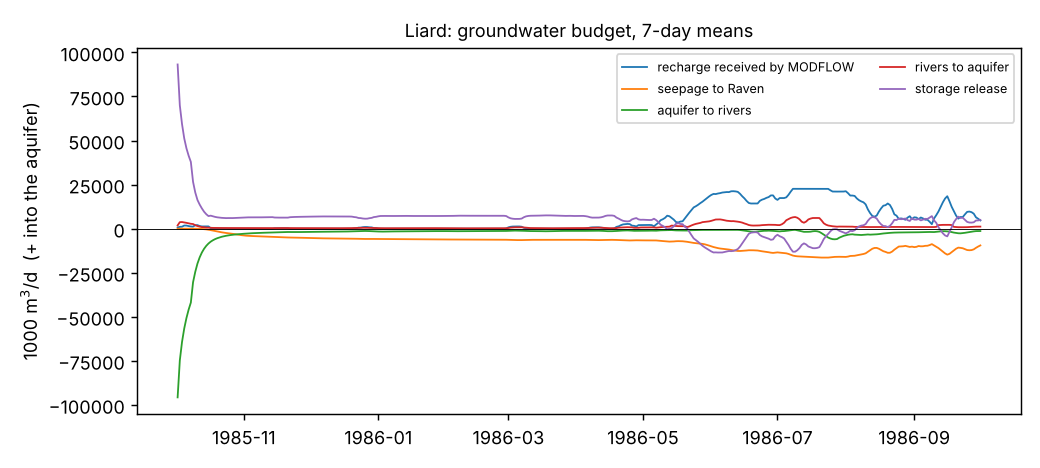
\includegraphics[width=0.9\linewidth]{figures/t1_gw_budget.png}
\caption{\cmd{gw\_budget.png}: the daily groundwater budget of the Liard example (7-day means; positive means into the
aquifer). The large flows of the first weeks are the aquifer adjusting from its initial heads (set by
\cmd{INITIAL\_HEAD\_DEPTH} in \cmd{Liard.rvp}). Afterwards, seepage and discharge to the rivers return the recharge, and
storage takes up the difference.}\label{fig:t1budget}\end{figure}
\begin{figure}[!htbp]\centering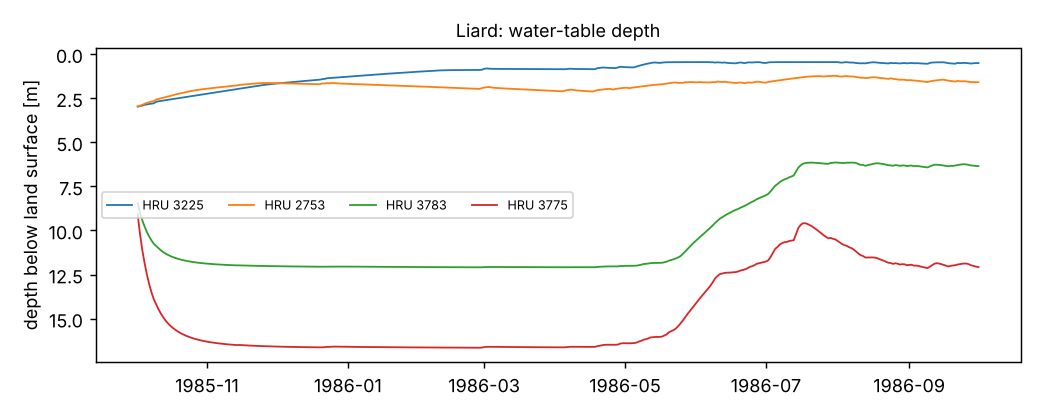
\includegraphics[width=0.9\linewidth]{figures/t1_gw_watertable.png}
\caption{\cmd{gw\_watertable.png}: water-table depth under the two shallowest and the two deepest HRUs. The option
\cmd{--hrus ID ...} of \cmd{plot\_gw.py} chooses other HRUs.}\label{fig:t1wt}\end{figure}
\begin{figure}[!htbp]\centering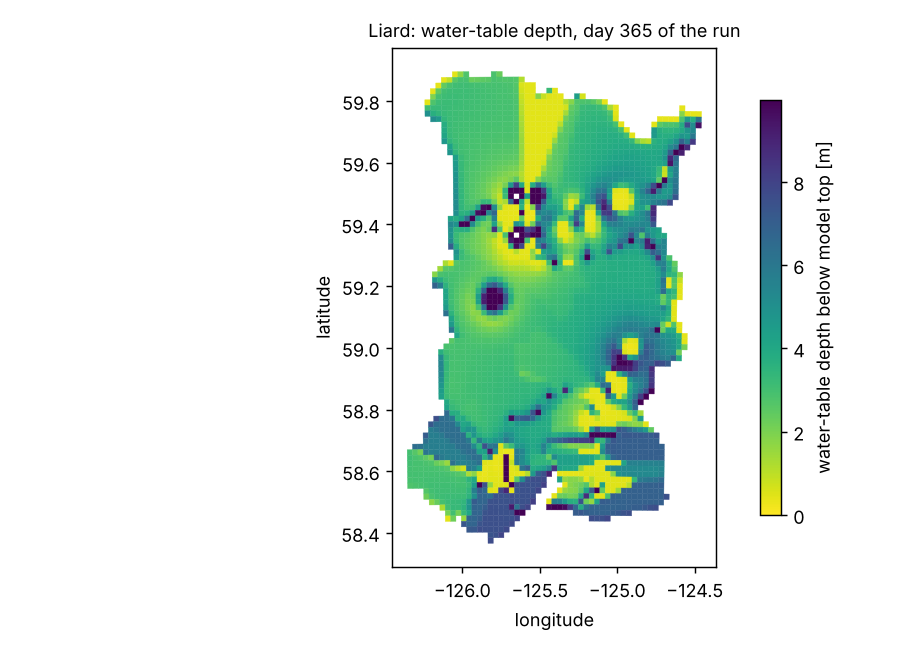
\includegraphics[width=0.72\linewidth]{figures/t1_gw_map.png}
\caption{\cmd{gw\_map.png}: water-table depth in every active column, at the last head field saved in
\cmd{out/mf6/gwf.hds}, on the cells of \cmd{out/mf6/grid\_cells.geojson}. The command \cmd{:HeadSaveFrequency} in
\cmd{Liard.rvg} sets how often MODFLOW saves the heads.}\label{fig:t1map}\end{figure}
\begin{trouble}
\cmd{ModuleNotFoundError: No module named \textquotesingle{}pandas\textquotesingle} (or numpy, matplotlib): the virtual environment is not active in this
terminal. Type \cmd{source \textasciitilde/raven-venv/bin/activate} (Step~\ref{st:python}).
\end{trouble}
\begin{note}[Reading MODFLOW's files yourself]
\cmd{out/mf6/gwf.hds} is a standard MODFLOW~6 head file and \cmd{gwf.dis.grb} its grid file. With FloPy,
\cmd{flopy.utils.HeadFile(\textquotesingle out/mf6/gwf.hds\textquotesingle).get\_data()} returns the last head field. \cmd{grid\_cells.geojson} holds
all cells in longitude and latitude, with their number and an \cmd{active} flag. It opens in any GIS program.
\end{note}
